\subsection{Melihat Daftar Pengguna}
Halaman ini hanya dapat diakses oleh \textit{administrator} yang sebelumnya sudah \textit{login}. Tidak ada \textit{view logic} ataupun logika \textit{UI} khusus dalam halaman ini. Kode sumber implementasi \textit{back-end} dapat dilihat pada Kode Sumber \ref{cdbe.05-01}.

\begin{figure}[h]
	\centering
	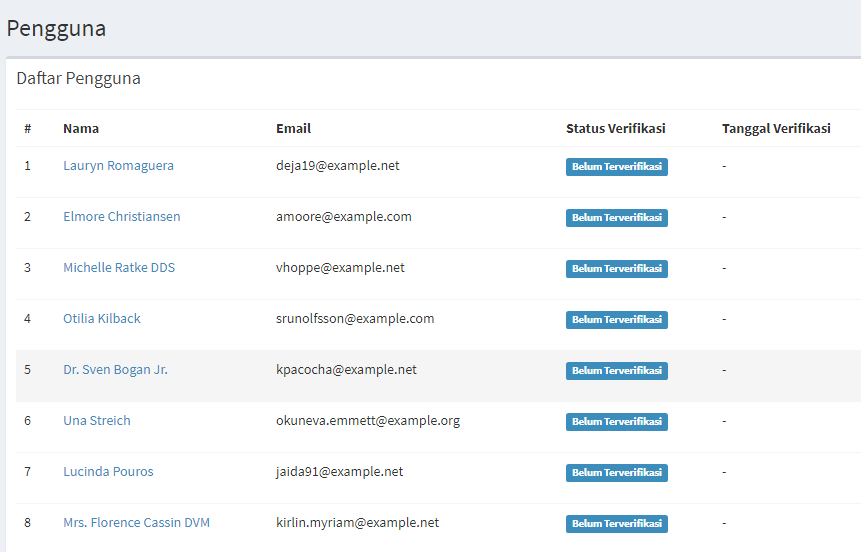
\includegraphics[width=.8\textwidth]{images/bab4/ui/05-01.png}
	\caption{Halaman Antarmuka Kasus Penggunaan Melihat Daftar Pengguna}
	\label{ui.05-01}
\end{figure}
\newpage
\begin{lstlisting}[label=cdbe.05-01,style=php,caption=Implementasi Antarmuka Melihat Daftar Pengguna]
/** 
 * File : app/Http/Controllers/UserController
 * Menampilkan halaman daftar pengguna
 * langsung diFetch dari base Model User
 * Method : GET
 */
public function user()
{
    $data['data'] = User::paginate(20);
    return view('pages.user.index', $data);
}
\end{lstlisting}


      
